\chapter{Hadoop}\label{cap:hadoop}
\noindent This chapter tries to expose with simplicity the defining fundamentals of Hadoop architecture. Initially abstract concepts will be introduced to give way to more particular and deep ideas that explore Hadoop implementation of the MapReduce model in two layers: the processing and the storage subsystem.

\section{The Beginnings}\label{sec:origen}
\noindent Hadoop roots its origins in \emph{Apache Nutch}, Mike Cafarella and Doug Cutting's implementation of an open source web index and search engine. Nutch project began in 2002. In spite of the Internet being notoriously smaller at the time, Nutch's underlying technology was unable to make it scale to manage the billion pages that comprised the \emph{old} Internet. But in 2003 Google publishes a research paper introducing \emph{GFS} (\emph{Google File System}) \cite{gfs}, a file system to be used across their clusters of commodity pcs that greatly simplified its deployment. Nutch will inherit a large part of the concepts detailed there translated in their own distributed file system implementation (\emph{NDFS}).

Also in 2004 appeared another publication \cite{googlemapreduce} that presented MapReduce, bringing about successive efforts to port Nutch algorithms to adapt to the emerging model. In mid 2005 most of Nutch code run following MapReduce guidelines over NDFS.

Both NDFS and Nutch MapReduce implementation were generic enough to be used without refactoring beyond web page indexing. In 2006 an unrelated project was constituted to extend Nutch's potentially reusable parts to widen their applicability context. This project was called Hadoop. In 2008 \emph{Yahoo!} announced that the index for their search engine in production was being continually refreshed by 10,000 Hadoop nodes. This same year Hadoop is brought out to the world becoming an Apache-backed project corroborating its success.

Nowadays, Hadoop is without doubt the MapReduce implementation most widely used by a broad range of companies.

\section{General Hadoop Architecture}\label{sec:arquitecturahadoop}
\noindent Hadoop composition differentiates four modules:
\begin{description}
 \item[Hadoop Common:] A module containing the parts used across the implementation. It is mainly comprised of scripts and configuration tools.
 \item[Hadoop MapReduce:] The module implementing the MapReduce processing model.
 \item[Hadoop YARN:] A general purpose framework abstracted from Hadoop MapReduce. It is employed to manage resources and schedule executions in distributed environments.
 \item[Hadoop DFS:] The distributed file system sustaining inputs and outputs from Hadoop clusters.
\end{description}

Hadoop architecture corresponds to the \emph{Master-Worker} archetype where two roles on each cluster appear: a unique Master and various Workers. These roles, and thus responsibilities, are fixed to different nodes by the cluster admin. If necessary, e.g. for maintenance, the admin may freely re-set the roles to new cluster nodes, only requiring job resubmissions if the Master role were reassigned.

This section will almost exclusively center around MapReduce and Hadoop DFS (HDFS) modules to expose the functionally covered with Hadoop. Hadoop YARN, as discussed, is a subsystem resulting from the isolation of scheduling and processing, both found together in the old --- pre Hadoop 2 --- MapReduce module, retaining task distribution and planning within YARN. This way, YARN is allowed to untie from Hadoop allowing for deployments where YARN orchestrates an implementation-agnostic working set. As of this writing, Hadoop YARN is still an alpha version.

Figures \ref{fig:hadoopmapredhdfs} and \ref{fig:hadoopmapreddfs} exhibit a high level vision of Hadoop architecture. Figure \ref{fig:hadoopmapredhdfs} shows an hypothetical deployment with HDFS. Figure \ref{fig:hadoopmapreddfs} shows a particular Hadoop installation with another supporting distributed file system.

\begin{figure}[tbp]
\begin{center}
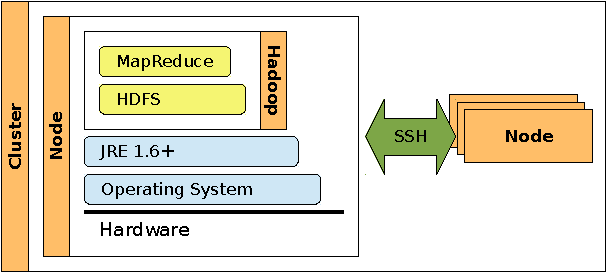
\includegraphics[width=0.7\textwidth]{imagenes/015.pdf}
 \caption{Hadoop over HDFS}
\label{fig:hadoopmapredhdfs}
\end{center}
\end{figure}

\begin{figure}[tbp]
\begin{center}
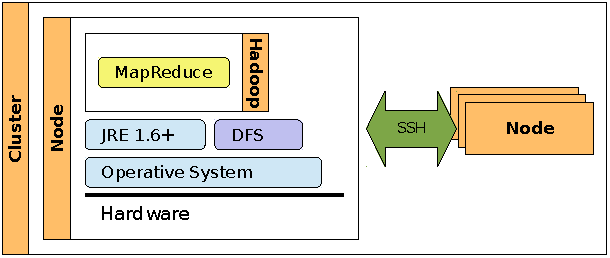
\includegraphics[width=0.7\textwidth]{imagenes/016.pdf}
 \caption{Hadoop over another DFS}
\label{fig:hadoopmapreddfs}
\end{center}
\end{figure}

From the figures it can be deduced that Hadoop runs atop a \emph{Java Virtual Machine} (emph{JVM}), that MapReduce requires a DFS implementation to rely on and that inter-node communication is conveyed through \emph{SSH} tunnels over TCP. Every module includes a web server (\emph{Jetty}) to ease collecting and reporting status information.

\section{Hadoop Distributed File System}\label{sec:hdfs}
\noindent HDFS has been designed to act as archival repository for huge masses of data whose main access pattern be \emph{write-one} \emph{read-many}. While it is no requisite for a data query to follow this access pattern, HDFS performance shines with read queries in batch mode. The underlying infrastructure, again, is composed by commodity pcs that HDFS manages to transform into a reliable, scalable, fault tolerant, self-balancing and network traffic reducing data store. Yet, as individual nodes are regular pcs, in HDFS converge some operating limitations:

\begin{itemize}
 \item High data access time. HDFS prioritizes large reads in batches and thus, reading small files is generally discouraged. As complement though, HDFS delivers \emph{very} high throughput by leveraging parallel reads on the cluster.
 \item High data writing time on many small files. Writing a file changes a block. Every file that be smaller than the HDFS block size must be persisted in a single block. That changed block must be send out across the network to keep the file system consistently updated. Thus, appending to many files requires updates in many blocks that would require synchronizing over the network.
 \item Multiple writes to the same file or ``\emph{not-append}'' operations are not supported. HDFS is not a \emph{POSIX}-compilant file system implementing only a set of operations to try to maximize data throughput in distributed environments.
\end{itemize}

To organize storage, HDFS takes from traditional operating systems the concept of block: an abstraction of the particular drive structure with a double purpose:

\begin{description}
 \item[Lowering DFS complexity:] Writing a block comprises storing data and meta-data, and handling information related to locate those data on disk. Using the block as the minimum organizational structure simplifies location expressions.
 \item[Incrementing flexibility:] files are free to grow over the size of an HDFS block.
\end{description}

To lay local drive blocks in position, HDFS makes use of two processes: the \emph{DataNode} and the \emph{NameNode}. Besides, as support, from Hadoop 0.21.0 onward it is permitted the optional deploying of a \emph{Backup Node} and a \emph{Checkpoint Node} in the same cluster.

\subsection{Node Roles}\label{subsec:rolesnodos}
\noindent Figure \ref{fig:desplieguehdfs} shows a layered down HDFS deployment. In dotted line appear both the Backup Node and the Checkpoint Node.

\begin{figure}[tbp]
\begin{center}
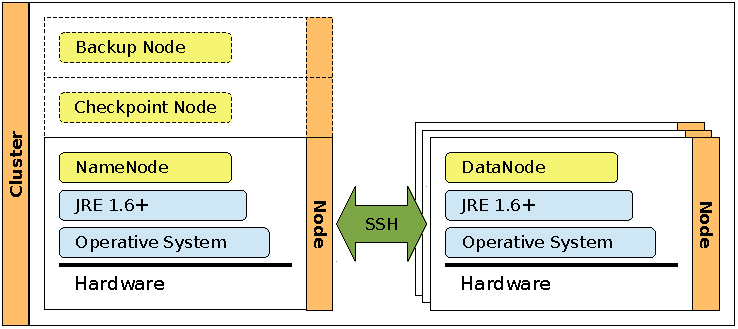
\includegraphics[width=0.85\textwidth]{imagenes/017.pdf}
 \caption{Typical HDFS deployment}
\label{fig:desplieguehdfs}
\end{center}
\end{figure}

\subsubsection{DataNode}\label{subsubsec:datanode}
\noindent DataNodes are those processes within nodes that handle the storage of HDFS blocks in their local drives. Every time a write to a file in a block succeeds, the DataNode in charge of the operation signals its supervising NameNode so that it could keep track the modifications to the DFS as they happen.

\subsubsection{NameNode}\label{subsubsec:namenode}
\noindent The NameNode is the process appointed to deal with the name space of the cluster. It has to handle the file system tree and meta-data that make possible recovering data from the DFS. It is such an important process that if it went down, every piece of data in HDFS would get lost, rendering impossible to match files with their container blocks. Therefore, the NameNode is seldom deployed with no Checkpoint Nodes or Backup Nodes in case the HDFS data were not stored elsewhere.

The information about the file system, meta-data, is persisted to the NameNode both in memory and disk. In this latter form, meta-data is managed in two files: one contains the name space of the file system as an image (\texttt{fsimage}), the other progressively appends the changes to the fsimage (\emph{edits}) as a log. When the DataNode starts, it compiles an fsimage afresh by merging the existing fsimage with the edits file. As soon as changes to the HDFS are reported from the NameNodes, the DataNode will update the edits log but without touching the fsimage. In a typical secured deployment, the edits file is kept in memory within the NameNode host computer, on the local file system and remotely via NFS.

\subsubsection{Checkpoint Node}\label{subsubsec:checkpointnode}
\noindent The Checkpoint Node is the means by which failure in the NameNode poses a smaller threat to the integrity of the data within HDFS. The idea behind the Checkpoint Node is to maintain a separate copy of the edits file so that it could periodically merge the fsimage with the edits, generating an updated fsimage to be uploaded to the NameNode. It should be noted that the Checkpoint Node does not listen to the network to record the modifications to the DFS in the edits file, it fetches the copy held by the NameNode itself. When the merging process be finished, the NameNode will be submitted the newly created fsimage, clearing out the old copy and reseting the edits file.

\subsubsection{Backup Node}\label{subsubsec:backupnode}
\noindent The Backup Node provides the same functionality as the Checkpoint Node by periodically creating restoration points of the name space but through a different approach. In this case, the Backup Node will download the fsimage file from the \emph{backed up} NameNode when booted, just like the Checkpoint Node, but it will receive notifications from the DataNodes on each modification to the HDFS, and will manage itself the merging between the fsimage and the edits file effectively creating a new fsimage, the same behavior as the NameNode.

Compared to the Checkpoint Node this process draws less bandwidth due to the fact that it does not require to download the fsimage nor the edits from the NameNode in order to stay synchronized.

The Hadoop version used in the VM of this project --- version 1.0.4 --- allows only a Backup Node per NameNode or multiple Checkpoint Nodes, not both. It should be noted that including a Backup Node in a cluster gives the possibility to run the NameNode with no persistent storage, i.e. with no allocated space in the local drive to write the fsimage and the edits, making the Backup Node the sole responsible for the duty.

\subsection{Network Topology}\label{subsec:topologiared}
\noindent One of the fundamental parts to a file system in a distributed environment is the capacity to provide a transparent mechanism by which information is persisted securely while, at the same, a certain amount of performance is maintained. HDFS makes use of an already discussed technique, \emph{replication}, that provides high performance, scalability and fault tolerance. Besides, HDFS has been devised to reduce the network congestion that stems from regular operation giving special emphasis to the way in which data is to be distributed in the cluster, controlling replica count or distance between replicas, among other variables, to concrete the block allocation policy.

\subsubsection{Node Distance}\label{subsubsec:distnodos}
\noindent To support the features that have been mentioned, it is fundamental for the NameNode to possess some information on the participating DataNodes physical location. With that information, the NameNode would be able to balance the \emph{physical distance} of the replicas, realizing that, generally, fault tolerance increases with replica distance but the bandwidth available to transfer replicas narrows. Thus, the NameNode will have to distribute the replicas across the cluster with a procedure that make the cluster safe without clogging the network.

To effectively calculate the physical distance between two replicas, the NameNode will use an approximate measure of the physical distance of the nodes storing the replicas. Therefore, the problem lies in finding a formula to calculate the distance between any two nodes in the cluster.

IP-based networks arrange participating nodes in an abstract tree structure that is simplified in four octets. Without deepening any further on this topic as it is clearly out of scope, it should be noted that, in properly configured networks, the closer two nodes are physically the smaller the distance between their respective routing gateways. This idea may be used recursively until the \emph{same} routing gateway was reached up from the initial nodes. So, the actual distance between two replicas is \emph{the number of steps required to find a common routing gateway, starting from the two nodes that stored the replicas}. The example below will clarify the procedure.

The way in which the NameNode calculates the distance among replicas lacks an  important feature that would render the cluster failure-prone. In order to keep HDFS fault tolerant, the NameNode has to deal with halting nodes, clogged networks, etc. If a stalled node were the gateway to a set of nodes, e.g the nodes in the same rack, then the access to any replica within that cluster would be impossible, and worse, if every replica of an individual block were stored in this rack, the block would be inaccessible for the duration of the outage in the gateway. Therefore, the distance alone cannot solve this distributing problems.

HDFS overcomes this limitations by mapping every IP address to a tuple with as many components as levels there were in the network --- typically three-tuples \emph{(data center, rack, node)}. Figure \ref{fig:distnodos} shows the most common values of the replica distance. With the help of the figure the procedure to get to $d=4$ will be succinctly explained.

The blue node holds the original block and the yellow one --- pointed by the $d=4$-labeled edge --- a replica. Both blocks are stored in nodes within the same data center but in different racks, thus, their nearest common ancestor gateway would be the one managing the routing between those two racks. Besides, every rack has an internal gateway that must be traversed in order for the internal traffic to exit the rack. So, each node would have to take \emph{2 steps} to get to their common gateway --- from node to \emph{in-rack} gateway to \emph{off-rack} gateway --- coming to \emph{4 steps}.

\begin{figure}[tbp]
\begin{center}
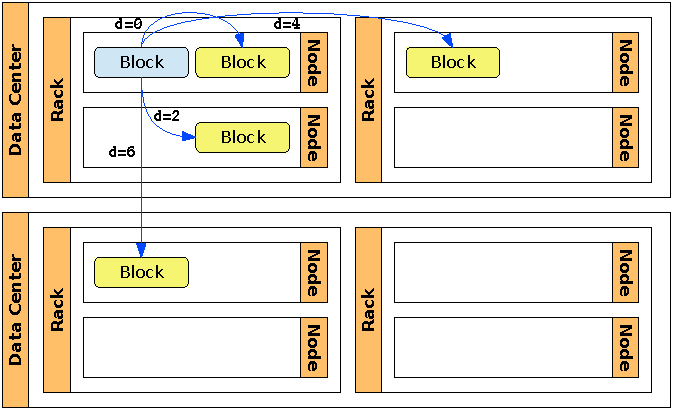
\includegraphics[width=0.75\textwidth]{imagenes/018.pdf}
 \caption{Replica distance}
\label{fig:distnodos}
\end{center}
\end{figure}

\subsubsection{Replication}\label{subsubsec:replicacionbloques}
\noindent Replication is a NameNode-controlled technique that relies on knowing the network topology to structure hierarchically the nodes in the cluster. Together with replica distance the NameNode is capable of enforcing a policy that balances data safety and throughput. What follows is the description of the method to distribute replicas over the cluster.

When a new block is written to HDFS --- or when an existing one is appended new data --- a configured number of replicas have to be made and distributed. By default, the NameNode will maintain updated three replicas of each block. The first block is placed in a node at random prioritizing those not too full nor too busy. Then, the first replica is stored in the same node as the original block. The second replica is sent off-rack to a node at random, and finally, the third replica is stored in the same rack as second but in a different node. If the \emph{replica factor} --- the total number of replicas every block will have --- were made higher, the successive replicas would be placed, again, in the same rack as the second one but in different nodes whenever possible.

This method provides the desirable equilibrium between fault tolerance (by assuring two copies of a block exist in different racks), consumed bandwidth (writing a new block would only need replicas to go through a single gateway as subsequent replicas are made within the rack), read performance (making it possible for every read request to be fulfilled from nodes in two racks) and balanced data distribution by executing the process just described. Figure \ref{fig:repbloque} exemplifies a factor 3 replication. The number in brackets indicates the order in which the replicas where created. The original block is the blue-colored one.

\begin{figure}[tbp]
\begin{center}
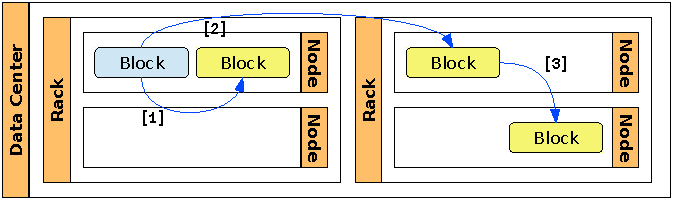
\includegraphics[width=0.75\textwidth]{imagenes/019.pdf}
 \caption{Replication factor 3}
\label{fig:repbloque}
\end{center}
\end{figure}


\section{Hadoop MapReduce}\label{sec:hadoopmapred}
\noindent In a typical Hadoop deployment, the execution module is lied over HDFS. This execution module is basically an implementation of the ideas exposed in the Google paper on MapReduce as a new programming paradigm \cite{googlemapreduce}. The core ideas that have been discussed for HDFS hold in this section, but with a different flavor. Hadoop MapReduce architecture is also based on the Master-Worker model and so appear two roles: a Master and a Worker.

The Master role is functionally covered by a process called the \emph{JobTracker}, whose main responsibility is task scheduling to workers. Complementarily, the worker role is implemented in the \emph{TaskTracker} which will actually execute the individual tasks reporting their progress back to the JobTracker.

\subsection{Node Roles}\label{subsec:rolesnodosmapred}
\noindent
\noindent La figura \ref{fig:desplieguehadoopmapred} representa un despliegue t\'ipico de Hadoop MapReduce en un cl\'uster, utilizando HDFS como sistema de ficheros distribuido soporte. Para completar la \emph{fotograf\'ia} habr\'ia que incluir los nodos responsables de gestionar el HDFS --- NameNode, Checkpoint Node y Backup Node --- omitidos por claridad.

\begin{figure}[tbp]
\begin{center}
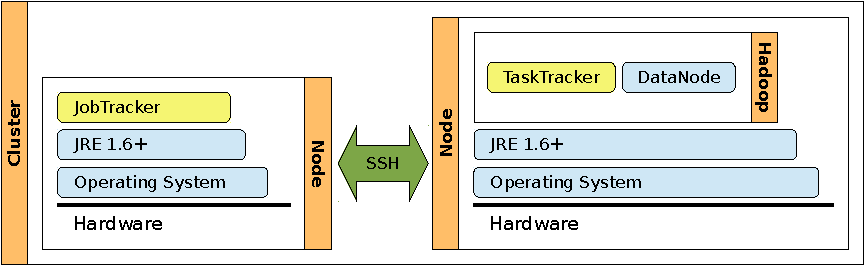
\includegraphics[width=0.99\textwidth]{imagenes/020.pdf}
 \caption{Ejemplo de despliegue de Hadoop MapReduce}
\label{fig:desplieguehadoopmapred}
\end{center}
\end{figure}

\subsubsection{JobTracker}\label{subsubsec:jobtracker}
\noindent El comportamiento del nodo JobTracker es muy similar al expuesto en el caso del NameNode de HDFS, pero aplicado a la gesti\'on de trabajos y tareas. Ante una petici\'on de ejecuci\'on, el JobTracker dividir\'a el trabajo asociado en tareas que repartir\'a entre los TaskTrackers que tenga bajo supervisi\'on. Normalmente, el tama\~no de los ficheros de entrada de las tareas se hace coincidir con el de los bloques del sistema de ficheros distribuido, sea o no HDFS, por ser lo m\'as eficaz. Para cerciorarse de que las ejecuciones concluyen con \'exito en un entorno expuesto al fallo, el JobTracker mantiene una lista de estado de las tareas asociadas a los nodos TaskTracker. De tal forma, en caso de que se produjese un error que impidiese la finalizaci\'on de alguna tarea, ya sea una tarea Map o una Reduce, el JobTracker replanificar\'ia su ejecuci\'on en otro nodo disponible con la m\'inima carga computacional.\newline

El reparto de trabajo se lleva a cabo siguiendo la m\'axima localidad, esto es, haciendo que los TaskTrackers reduzcan tareas basadas en la transformaci\'on de datos almacenados en el mismo nodo. As\'i se reducen tanto el tiempo de acceso al dato del TaskTracker, como la saturaci\'on de la red del cl\'uster, haciendo la computaci\'on m\'as ligera.\newline

Tal y como suced\'ia en la definici\'on general del MapReduce de Google \cite{googlemapreduce}, el fallo en un JobTracker es muy problem\'atico porque s\'olo est\'a cubierta la posibilidad de correr uno por cl\'uster sin usar herramientas adicionales. Dada una ca\'ida en el JobTracker, el procedimiento de recuperaci\'on ``resuelve'' la situaci\'on descartando los trabajos sin concluir; esperando que el nuevo JobTracker pueda hacerse cargo del procesado de esos trabajos incompletos que habr\'an de ser enviados manualmente por los usuarios. Actualmente s\'i se pueden manejar JobTrackers adicionales en un mismo cl\'uster e instante temporal usando una herramienta adicional: \emph{Zookeeper}.


\subsubsection{TaskTracker}\label{subsubsec:tasktracker}
\noindent La misi\'on fundamental del TaskTracker es procesar las tareas que le sean enviadas desde el JobTracker. Peri\'odicamente, el TaskTracker env\'ia una se\~nal a su JobTracker para informar acerca del estado de progreso de la ejecuci\'on de una tarea, si tuviese una asignada, o para indicar que se encuentra a la espera. Si el JobTracker no recibiese esa se\~nal en un intervalo convenido, \'este marcar\'ia el TaskTracker y \emph{todas} sus tareas relacionadas ---las concluidas y las incompletas--- como inaccesibles. Esta clase de fallo, es decir la ca\'ida de un TaskTracker, se considera menos problem\'atico que en el caso del JobTracker, pero implica replanificaci\'on de tareas e incluso repetici\'on de la ejecuci\'on de alguna. Usando la comentada lista de estado de las tareas, el JobTracker buscar\'a las inaccesibles necesarias ---las Map completadas y las Reduce cuya salida no est\'e en el DFS--- y har\'a la redistribuci\'on siguiendo la mec\'anica descrita.
